\documentclass[a4paper]{article}

\usepackage{tabularx}
\usepackage[portuguese]{babel}
\usepackage[utf8]{inputenc}
\usepackage{indentfirst}
\usepackage{graphicx}
\usepackage{verbatim}
\usepackage{wrapfig}
\usepackage{booktabs}
\usepackage{placeins}
\usepackage{listings}
\usepackage{color}

\definecolor{dkgreen}{rgb}{0,0.6,0}
\definecolor{gray}{rgb}{0.5,0.5,0.5}
\definecolor{mauve}{rgb}{0.58,0,0.82}
\graphicspath{ {./img/} }

\begin{document}

\setlength{\textwidth}{16cm}
\setlength{\textheight}{22cm}

\title{\Huge\textbf{Adaptoid}\linebreak\linebreak\linebreak
\Large\textbf{Relatório Final}\linebreak\linebreak
\linebreak\linebreak

\includegraphics[scale=0.1]{feup-logo.png}\linebreak\linebreak
\linebreak\linebreak
\Large{Mestrado Integrado em Engenharia Informática e Computação} \linebreak\linebreak
\Large{Programação em Lógica}\linebreak
}

\author{\textbf{Grupo 04 : Adaptoid}\\ David Azevedo - 201405846 \\ João Ferreira - 201404332 \\\linebreak\linebreak \\
 \\ Faculdade de Engenharia da Universidade do Porto \\ Rua Roberto Frias, s\/n, 4200-465 Porto, Portugal \linebreak\linebreak\linebreak
\linebreak\linebreak\vspace{1cm}}
\date{Novembro de 2016}
\maketitle
\thispagestyle{empty}

%************************************************************************************************
%************************************************************************************************

\newpage

\section*{Resumo}
O problema abordado consitiu na implementação do jogo de tabuleiro "Adaptoid" na linguagem Prolog, o que nos representou como sendo um novo desafio, visto que, o grupo não estava familiarizado com este paradigma de programação em lógica. Os objectivos do projecto incluiram : permitir três modos de utilização (Humano/Humano, Humano/Computador, Computador/Computador), incluir dois níveis de jogo para o computador, interface adequada em modo de texto. O trabalho foi elaborado com base em 5 passos fundamentais implementados pela seguinte ordem :
\begin{enumerate}
    \item Representação do tabuleiro em Prolog usando códigos ASCII.
    \item Implementação das regras do jogo em predicados lógicos.
    \item Criação de uma interface simples com o utilizador.
    \item Desenvolvimento de uma pseudo AI para as jogadas do computador.
    \item Design de um sistema simples de menus para completar um ambiente de jogo.
\end{enumerate}

Todos os objectivos foram cumpridos sendo que temos um jogo completo e jogável desenvolvido em Prolog. Desenvolver um jogo funcional numa linguagem nova com a qual apenas se teve contacto durante algumas semana não é fácil, pelo que o grupo no inicio encontrou algumas dificuldades. Após uma leitura extensiva dos slides facultados pelos docentes assim como informação disponível na web foi possível obter uma melhor percepção desta linguagem e paradigma de programação por forma a desenvolver uma aplicação.


Concluindo, ambos os estudantes orgulham-se agora do resultado obtido e do método como tal foi alcançado, podemos também afirmar que o nosso conhecimento de Prolog aumentou consideravelmente.
\newpage

\tableofcontents

%************************************************************************************************
%************************************************************************************************

%*************************************************************************************************
%************************************************************************************************

\newpage

%%%%%%%%%%%%%%%%%%%%%%%%%%
\section{Introdução}

Este projecto foi proposto no âmbito da unidade curricular de Programação em Lógica do Mestrado Integrado de Engenharia Informática e de Computação. Consiste na adaptação de um jogo de tabuleiro para dois jogadores na linguagem Prolog. O tema escolhido foi o "Adaptoid" um jogo relativamente simples de compreender e aprender a jogar, mas que a quantidade de opções disponíveis ao jogador fazem com que o jogo tenha uma complexidade muito superior relativa ao que aparenta.
Este relatório tem a seguinte estrutura :
 \begin{itemize}
   \item Descrição do jogo, a sua história e regras.
   \item Implementação da lógica do jogo em Prolog.
   \item Forma de representação do estado do tabuleiro e sua visualização.
   \item Execução de movimentos.
   \item Verificação do cumprimento das regras do jogo.
   \item Determinação do final do jogo.
   \item Cálculo das jogadas a realizar pelo computador.
   \item Módulo de interface com o utilizador em modo de texto.
   \item Conclucões.
   \item Bibliografia.
   \item Anexos.
 \end{itemize}

\newpage
%%%%%%%%%%%%%%%%%%%%%%%%%%
\section{O Jogo Adaptoid}

\begin{wrapfigure}{r}{0.22\textwidth}
    \centering
    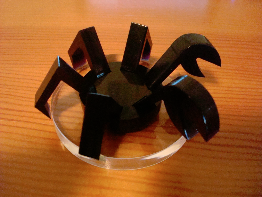
\includegraphics[width=0.22\textwidth]{adaptoid}
    \caption{Imagem ilustratica de um "adaptoid"}
\end{wrapfigure}

Adaptoid é um jogo de tabuleiro para dois jogadores, constituído por um tabuleiro hexagonal, que contém (37 espaços), e por um conjunto de criaturas denominadas de “adaptoid”. Cabe a cada jogador evoluir o seu “adaptoid” adicionando membros, garras e pernas, ao corpo do adaptoid. Os membros são fatores decisivos, pois fazem variar o comportamento do “adaptoid”. As garras definem o dano e as pernas a capacidade de movimento.

\begin{wrapfigure}{l}{0.20\textwidth}
    	\centering
	\vspace{-10pt}
   	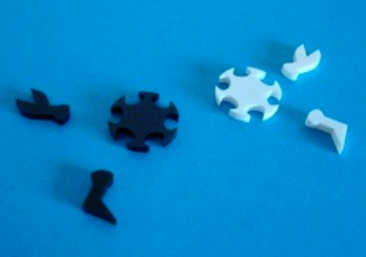
\includegraphics[width=0.20\textwidth]{adaptoidsDissecados}
    	\caption{Corpo e membros de um "adaptoid"}
\end{wrapfigure}

Cada turno divide-se em 3 fases distintas, sendo elas, movimento, crescimento e alimentação. Durante a fase de movimento o jogador pode mover um dos seus “adaptoids”, o número de espaços percorridos depende do número de pernas desse “adaptoid”.

Não é possível mover o adaptoid através de espaços que estejam ocupados, apenas é possível mover em direção a espaços vazios sem obstáculos e mover para o topo de um “adaptoid” oposto, para iniciar a captura. Na fase de crescimento o jogador pode optar por um de dois casos possíveis, ou cria um novo corpo adjacente a um dos seus “adaptoids” existentes, ou então adiciona uma perna, ou garra, a um dos seus “adaptoids” existentes no tabuleiro. Na fase de alimentação, é verificada em cada peça do inimigo se ela está com fome, ou seja, o número  de espaços vazios à sua volta terá que ser igual ou maior ao número de membros do “adaptoid”. No caso de fome, a peça inimiga morre, é removida e é atribuído um ponto ao jogador. Durante a captura o “adaptoid ”com mais garras ganha e o “adaptoid ” derrotado é removido do tabuleiro. Em caso do número de garras dos “adaptoids” ser igual, ambos são removidos e cada jogador recebe um ponto. As peças de “adaptoids” mortos poderão ser novamente usadas. O jogo termina quando um jogador chega aos 5 pontos ou quando um dos jogadores ficar sem nenhum “adaptoid” no tabuleiro.


\begin{figure}[h]
    \begin{center}
        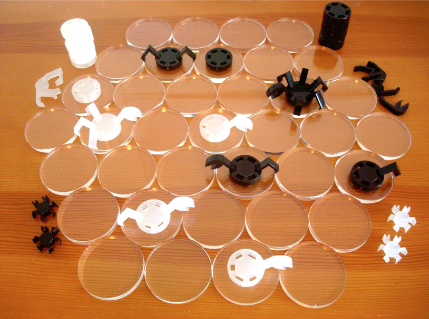
\includegraphics[scale=0.5]{jogoDecorrer}
        \caption{Estado de um jogo de adaptoid}
        \centering
    \end{center}
\end{figure}

\newpage
%%%%%%%%%%%%%%%%%%%%%%%%%%
\section{Lógica do Jogo}

\subsection{Representação do Estado do Jogo}  Para representar o tabuleiro do jogo optámos por uma lista de listas, onde cada uma das listas define uma das linhas do tabuleiro e por consequência cada elemento dessa lista representa uma célula no nosso jogo,  para facilitar a pesquisa de casas adjacentes foi inserido no início de cada lista alguns átomos que mais tarde serão interpretados como espaços por forma a garantir a forma hexagonal definida pelos criadores do jogo. As peças do jogo, os “adaptoids”, são representados usando uma lista de 4 elementos ([Id,Cor,NPernas,NGarras]). Os ID têm como função facilitar na pesquisa das peças no tabuleiro. A Cor assume o valor ‘O’(white) ou ‘X’(black), e representa o jogador ao qual a peça pertence, uma vez que na consola do sicstus não é possível alterar a cor. O NPernas como o nome indica é o número de pernas que a peça possui, idem para o NGarras.

\begin{figure}[h]
    \begin{center}
        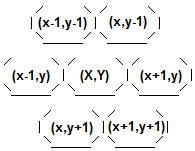
\includegraphics[scale=0.5]{posicoesRelativas}
        \caption{Posições relativas a uma célula central}
        \centering
    \end{center}
\end{figure}
Nota: Os átomos ‘a’,’b’,’c’,'d','e','f','g' e ‘\#’ são usados para controlar a posição das casas do jogo relativa à lista que representa a linha do tabuleiro onde estas se encontram, ou seja, com a introdução destes símbolos é possível seguir a seguinte lógica: Para uma determinada célula na posição (x,y), a célula-vizinha imediatamente abaixo do lado esquerdo está na posição (x,y+1) e a célula imediatamente abaixo do lado direito está na posição (x+1,y+1). Neste pequeno exemplo, o jogador da equipa ‘X’(white) ganhou porque o jogador da equipa ‘O’(black) não possui mais nenhuma peça no tabuleiro. Também é possível ambos os jogadores terem peças no tabuleiro e um ganhar, mas neste caso o jogador vencedor alcançou primeiro os 5 pontos.



\newpage

\subsection{Visualização do Tabuleiro} Originalmente as células do tabuleiro são redondas, mas para efeitos de visualização utilizando caracteres ASCII, estas são representadas como hexágonos. Com este formato, para ser possível o desenho do “adaptoid” contendo as suas garras e pernas seguiu-se a seguinte estratégia: Nesta célula é possível observar todas as posições possíveis para as garras(símbolo Y ) e pernas(símbolo L), este caso é impossível já que o número máximo de membros é 6, mas para efeitos de demonstração do funcionamento, é possível observar que as garras(Y) são desenhadas apenas no topo e no meio (caso sejam 6 garras no total), o mesmo acontece para as pernas. O símbolo B representa a cor do “adaptoid” e à sua volta está o número dessa peça.
Para que o desenho de cada célula seja possível, para cada linha do conteúdo do tabuleiro são desenhadas 4 linhas no ecrã, sendo elas:

\begin{table}[h!]
  \centering
  \caption{Legenda das camadas de uma célula.}
  \label{tab:table1}
 \newcolumntype{P}[1]{>{\centering\arraybackslash}p{#1}}
  \begin{tabular}{ c |  P{9.8cm}}
	\hline &
	\\
	
\includegraphics[width=0.1\textwidth]{topo}
           & A linha de topo que contém o número de garras (até 5 garras).
	\\&
	\\

	
\includegraphics[width=0.1\textwidth]{meio}
	& A linha do meio que contém o sexto membro (garra/perna), a cor e  número da peça.
	\\

	
\includegraphics[width=0.1\textwidth]{baixo}
	& A linha de baixo que contém o número de pernas (até 5 pernas).

	\\
	
\includegraphics[width=0.06\textwidth]{separacao}
	& A linha de separação para ser possível uma melhor distinção entre células adjacentes.
	\end{tabular}
\end{table}
\FloatBarrier
Foram utilizados símbolos especiais que apenas são usados como espaçamento, para que seja possível enquadrar as células no seu local. O predicado de visualização já se encontra 100\% desenvolvido sendo que recebe um tabuleiro no formato de lista de listas e procede ao desenho no mesmo na consola como se pode ver na figura ao lado.

\subsection{Lista de Jogadas Válidas}Foram implementados predicados que definem as jogadas válidas, estes predicados implementam as jogadas propriamente ditas e validam no caso do utilizador, no caso do computador são usados para obter a lista de jogadas possíveis. As três regras que se seguem dizem respeito às diferentes fases de que cada jogada (Movimento(M), Evolução(E) e Alimentação(famintos)).
\begin{itemize}
    \item \textit{lerRegraM(+Cor,+Acao,+JogoInicial,-JogoFinal)} , as ações possíveis incluem \textit{mover(+X,+Y,+Ori)} e \textit{capturar(+X,+Y,+Ori)}.
    \item \textit{lerRegraE(+Cor,+Acao,+JogoInicial,-JogoFinal)} , as ações incluem \textit{aP(+X,+Y)} para adicionar uma perna, \textit{aG(+X,+Y)} para adicionar uma garra e \textit{aC(+X,+Y,+Ori)} para adicionar um novo adaptoid.
    \item \textit{famintos(+JogoInicial,+Cor,-JogoFinal)}.
\end{itemize}

\newpage

\subsection{Execução de Jogadas} Validação e execução de uma jogada num tabuleiro, obtendo o novo estado do jogo. Exemplo: \textit{move(+Move, +Board, -NewBoard)}.
\begin{itemize}
    \item \textit{capturar(+JogoInicial, +ID, +Cor, +Ori, -JogoFinal)}.
    \item \textit{moverPeca(+JogoInicial, +ID, +Cor, +Ori, -JogoFinal)}.
    \item \textit{addPerna(+Board, +Cor, +ID, -NewBoard)}.
    \item \textit{addGarra(+Board, +Cor, +ID, -NewBoard)}.
    \item \textit{addCorpo(+Board, +ID, +Cor, +Ori, -NewBoard)}.
    \item \textit{esfomeados(+OriginalBoard, +BoardCopy, +Cor, -Nremovidos, -NewBoard)} esta função não é usada diretamente pelo utilizador mas é feita no final de cada jogada.
\end{itemize}

\subsection{Avaliação do Tabuleiro}\label{evalTab}

A avaliação do estado do jogo é realizada no predicado  \textit{getValue(+JogoI, +Cor,+Pos, -Value)}, este predicado internamente usa outros predicados de avaliação, para que promova certos movimentos. Estes predicados são:

\begin{itemize}
    \item \textit{getValueByPoints(+JogoI, +Cor, +Pos, -Value, +M)}. Atribui um valor dependendo os pontos ganhos nessa jogada, sendo M a pontuação.
    \item \textit{getValueByPecas(+JogoI, +Cor, +Pos, -Value, +M)}. Atribui um valor dependendo do número de peças , sendo M a pontuação.
    \item \textit{getValueByStarving(+JogoI, +Cor, +Pos, -Value, +M)}. Atribui um valor dependendo do número de peças que possam ser perdidas posteriormente devido à condição de fome, sendo M a pontuação.
    \item \textit{getValueByPernas(+JogoI, +Cor, +Pos, -Value, +M1, +M2)}. Atribui um valor dependendo do número de garras e o número de adaptoids com garras, sendo M1 a pontuação de elementos com pernas e M2 o numero total de pernas.
    \item \textit{getValueByGarras(+JogoI, +Cor, +Pos, -Value, +M1, +M2)}. Atribui um valor dependendo do número de garras e o número de adaptoids com garra, sendo M1 a pontuação de elementos com garras e M2 o numero total de garras.
    \item \textit{getValueByMovimento(+JogoI, +Cor, +Pos, -Value, +M)}. Atribui um valor dependendo do número de pernas e o número de adaptoids com pernas, sendo M a pontuação.
    \item \textit{getValueByCloser(+JogoI, +Cor, +Pos, -Value, +M)}. Atribui um valor dependendo da próximidade e possibilidade de ataque a um inimigo, sendo M a pontuação.
\end{itemize}

\subsection{Final do Jogo} Foi criado o predicado \textit{ganhou(-Jogador,+Jogo)} que avalia se um dado jogo chegou ao fim, verificando as seguintes condições : algum dos jogadores alcançou os 5 pontos ou algum dos jogadores não possuí peças no tabuleiro. Este predicado é chamado em duas ocasiões, a primeira, no fim de cada jogada simplesmente para saber se o jogo terminou, ou seja, se existe um vencedor, e uma segunda vez após ter terminado o \textit{loop} de jogar para se obter o estado de terminação (jogador vencedor ou empate) de forma a imprimir o resultado.

\subsection{Jogada do Computador}
A escolha da melhor jogada é feita no predicado:
\begin{itemize}
	\item \textit{escolheMelhorJogada(+JogoI,+Cor,+Modo,-JogoF)}.
\end{itemize}

O modo determina o nível de dificuldade do computador, tendo como opções disponíveis um modo de ataque (\textit{op}) e um modo de defesa (\textit{notOP}). Internamente o modo alterna entre \textit{getValue} e \textit{getValue2} que apenas mudam os multiplicadores para obter comportamentos diferentes. A forma como são escolhidas as opções já foi mencionada na secção~\ref{evalTab}.

\subsection{Testes}

Foram realizados testes durante a fase de desenvolvimento da lógica do jogo, para garantir a funcionalidade dos predicados implementados e o cumprimento das regras.

Estes testes apenas abrangem a parte lógica do projeto uma vez que é considerada como sendo a componente mais critica do projeto. O que implica que terá de ser, por conseguinte, a parte mais robusta.


%%%%%%%%%%%%%%%%%%%%%%%%%%
\newpage
\section{Interface com o Utilizador}

O módulo de interface principal divide-se em vários predicados sendo que cada um indica um menu. Este design foi desenvolvido a pensar no utilizador, para que seja possivel uma navegação mais intuitiva entre os menus.
\begin{figure}[h]
    \begin{minipage}[b]{0.4\textwidth}
        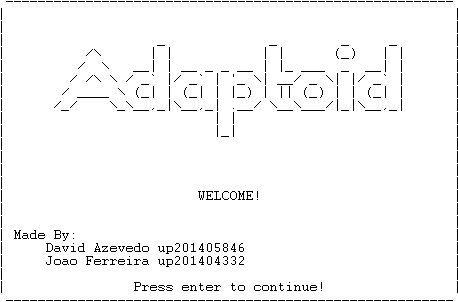
\includegraphics[scale=0.5]{menuPrincipal}
        \caption{Menu de início.}
    \end{minipage}
    \begin{minipage}[b]{0.4\textwidth}
        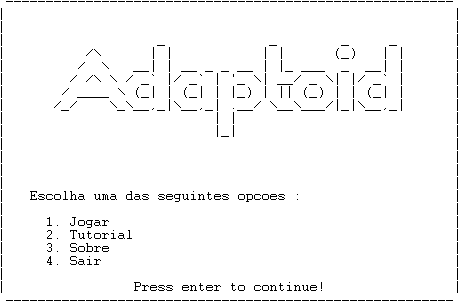
\includegraphics[scale=0.5]{menuEscolha}
        \caption{Menu principal.}
    \end{minipage}
\end{figure}


Os menus que o utilizador pode encontrar contêm:

\begin{itemize}
	\item Instruções (tutorial).
	\item Especificação do jogo.
	\item Escolha do tipo de jogo.
	\item Escolha da dificuldade do computador.
\end{itemize}

\begin{figure}[h]

    	\centering
     	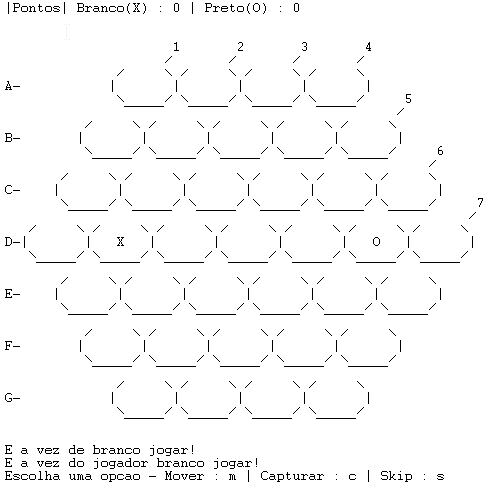
\includegraphics[scale=0.5]{ingame1}
	\caption{Menu de jogo.}
	\label{fig:figuramenu}

\end{figure}
No modo humano contra humano ou humano contra computador, durante a jogada do utilizador, é apresentado um menu como o indicado na figura~\ref{fig:figuramenu}, indicando os passos que o utilizador deverá seguir para realizar a sua jogada.

Em modo computador contra computador, é apresentado ao utilizador o tabuleiro do resultado de cada ronda, sendo necessária a interação do utilizador para proceder à próxima ronda, terminando com um texto indicativo do resultado final.



%%%%%%%%%%%%%%%%%%%%%%%%%%
\newpage
\section{Conclusões}
O grupo vê positivamente o resultado final que obteve e os conhecimentos adquiridos durante o desenvolvimento do projeto. Reconhecemos que a linguagem Prolog é bastante útil para a resolução de problemas relacionados com lógica, como era o caso deste mesmo jogo de tabuleiro, entre outros problemas do mundo real. Nunca é demais lembrar o peso e o significado destes problemas, uma vez que o modelo estrutural aqui representado pode-nos levar a considerar a reestruturação dos modos de operação convencionais.
\\

O jogo Adaptoid mostrou-nos que apesar da sua simplicidade consegue ser um jogo bastante apelativo e um bom exercício cerebral.
\\

Foram encontradas algumas dificuldades durante a realização deste trabalho que com o auxilio do material disponibilizado pelos docentes, e ainda o material que se encontra online, foram possiveis de ser ultrapassados. Inicialmente não foi um projeto que nos apelou muito devido a ser um estilo "relativamente" novo de programação e ao qual não estamos habituados, isto significa que, durante os primeiros dias de impletamentação o grupo esteve um pouco perdido e sem saber o que fazer. Optámos por utilizar uma tarde somente na pesquisa de informação sobre o Prolog (de notar que este tempo foi reduzido devido às informações e dicas já apresentadas nas aulas teóricas). Após este periodo de adaptação, os estudantes conseguiram resolver o problema proposto de uma forma ágil, dedicada, empenhada e acima de tudo correta.
\\

Na nossa opinião, é importante referir que o modo de \textit{input} não ficou da forma que o grupo mais gostaria, mas uma vez que é necessário tratar situações de erro humano achamos que a opção escolhida, apesar de não ser a mais funcional, é a mais robusta. Outro aspeto importante é a inteligência artificial, mas esta parte não recebeu uma importância tão elevada devido a ser alvo de estudo no próximo semestre.
\\

Concluindo, foi um projeto bastante interessante e educativo que nos abriu novos horizontes no mundo da programação em lógica, ambos os estudantes estão gratos pela experência e orgulhosos pelo seu resultado.

\clearpage
%\addcontentsline{toc}{section}{Bibliografia}
%\renewcommand\refname{Bibliografia}
%\bibliographystyle{plain}
%\bibliography{myrefs}

\newpage
\appendix
\section{adaptoid.pl}
\lstset{frame=tb,
  language=Prolog,
  aboveskip=3mm,
  belowskip=3mm,
  showstringspaces=false,
  columns=flexible,
  basicstyle={\small\ttfamily},
  numbers=none,
  numberstyle=\tiny\color{gray},
  keywordstyle=\color{blue},
  commentstyle=\color{dkgreen},
  stringstyle=\color{mauve},
  breaklines=true,
  breakatwhitespace=true,
  tabsize=3
}
\begin{lstlisting}
:- use_module(library(lists)).
:- include('tabuleiro.pl').
:- include('testes.pl').
:- include('logic.pl').
:- include('utils.pl').
:- include('ai.pl').
:- include('menu.pl').

%Predicado que inicia o jogo criando um tabuleiro com as posicoes iniciais e a instancia jogo com ambos os pontos a 0 e o novo tabuleiro criado
init :- write('Comecando o jogo!'),tabuleiro(Tab), asserta(jogo(0,0,Tab)), nl.
%Predicado para terminar e eliminar a instancia de jogo
end :- retract(jogo(_,_,_)), write('Fim do Jogo!'), nl.

%Predicados de desenho do jogo
desenharJogo(A,B,Tab) :- clearScreen, write('|Pontos| Branco(X) : '), write(A), write(' | Preto(O) : '), write(B), nl, desenharTabuleiro(Tab).
desenharJogo(jogo(A,B,Tab)) :- desenharJogo(A,B,Tab).

%Predicados para imprimir o resultado do jogador
imprimeVencedor(branco):- write('Jogador Branco Ganhou! Parabens!'), nl.
imprimeVencedor(preto):- write('Jogador Preto Ganhou! Parabens!'), nl.
imprimeVencedor(empate):- write('Ninguem Ganhou! Empate!'), nl.
imprimeVez(Cor):- write('E a vez do jogador '), write(Cor), write(' jogar!'), nl.

%Predicado para a jogada do jogador branco
jogadaBranco(Jogo,Jogo) :- ganhou(_,Jogo).
jogadaBranco(jogo(A,B,Tab),jogo(A1,B1,T1)) :-   desenharJogo(A,B,Tab),
                                             write('E a vez de branco jogar!'), nl,
                                             jogada(jogo(A,B,Tab),branco,jogo(A1,B1,T1)).

%Predicado para a jogada do jogador preto
jogadaPreto(Jogo,Jogo) :- ganhou(_,Jogo).
jogadaPreto(jogo(A,B,Tab),jogo(A1,B1,T1)) :-    desenharJogo(A,B,Tab),
                                             write('E a vez de preto jogar!'), nl,
                                             jogada(jogo(A,B,Tab),preto,jogo(A1,B1,T1)).

%Predicados que representam uma ronda do jogo
jogando(hh,Jogo) :- retract(jogo(A,B,Tab)), !,
                 jogadaBranco(jogo(A,B,Tab),jogo(A1,B1,T1)), !,
                 jogadaPreto(jogo(A1,B1,T1),jogo(A2,B2,T2)),
                 asserta(jogo(A2,B2,T2)), Jogo = jogo(A2,B2,T2).
jogando(hh,_).
jogando(hOp,Jogo) :- jogando(hc,op,Jogo).
jogando(hRe,Jogo) :- jogando(hc,notOp,Jogo).
jogando(opOp,Jogo):- jogando(cc,Jogo,op,op).
jogando(opRe,Jogo):- jogando(cc,Jogo,op,notOp).
jogando(reRe,Jogo):- jogando(cc,Jogo,notOp,notOp).
jogando(hc,M,Jogo) :- retract(jogo(A,B,Tab)), !,
                 jogadaBranco(jogo(A,B,Tab),jogo(A1,B1,T1)), !,
                 jogadaComputador(preto,M,jogo(A1,B1,T1),jogo(A2,B2,T2)),
                 desenharJogo(A2,B2,T2),
                 asserta(jogo(A2,B2,T2)), Jogo = jogo(A2,B2,T2).
jogando(hc,_,_).
jogando(cc,Jogo,M1,M2) :- retract(jogo(A,B,Tab)), !,
                 jogadaComputador(branco,M1,jogo(A,B,Tab),jogo(A1,B1,T1)),
                 jogadaComputador(preto,M2,jogo(A1,B1,T1),jogo(A2,B2,T2)),
                 desenharJogo(A2,B2,T2), write('Prima /*|ENTER|*\\'), get_char(_),
                 asserta(jogo(A2,B2,T2)), Jogo = jogo(A2,B2,T2).
jogando(cc,_,_,_).

%Loop do Jogo
jogar(Modo) :- init, repeat, once(jogando(Modo,Jogo)), ganhou(Jogador,Jogo), desenharJogo(Jogo), imprimeVencedor(Jogador), end.

%Representa uma jogada individual
jogada(jogo(A,B,Tab),Cor,jogo(A3,B3,T3)):-  imprimeVez(Cor), !, repeat,
                                         movimento(jogo(A,B,Tab),Cor,jogo(A1,B1,T1)),
                                         desenharJogo(A1,B1,T1), !, repeat,
                                         evoluir(jogo(A1,B1,T1),Cor,jogo(A2,B2,T2)), !,
                                         famintos(jogo(A2,B2,T2),Cor,jogo(A3,B3,T3)).

%Predicado para ler a opcao de movimento
movimento(JI,Cor,JF) :- write('Escolha uma opcao - Mover : m | Capturar : c | Skip : s'), nl, !,
                     read(X), acao1(JI,X,Regra), !, lerRegraM(Cor,Regra,JI,JF).
lerRegraM(_,s,Jogo,Jogo).
lerRegraM(Cor,mover(X,Y,Ori),jogo(A,B,Tab),jogo(A,B,T1)) :- getSimboloXY(Tab,[ID,Cor,_,P],X,Y), P > 0,
                                                         validarOri(Ori,P),
                                                         moverPecaLista(Tab,ID,Cor,Ori,T1).
lerRegraM(Cor,capturar(X,Y,Ori), jogo(A,B,Tab), JF) :-  getSimboloXY(Tab,[ID,Cor,G,_],X,Y),
                                                     G > 0,
                                                     capturar(jogo(A,B,Tab),ID,Cor,Ori,JF).

%Predicado para ler a opcao de evolucao
evoluir(Jogo,_,Jogo):- ganhou(_,Jogo).
evoluir(JI,Cor,JF) :-   write('Escolha um opcao - Adicionar Perna : p | Adicionar Garra : g | Adicionar Corpo : c | Skip : s'), nl , !,
                     read(Acao), acao2(Acao,Regra), !, lerRegraE(Cor,Regra,JI,JF).
lerRegraE(_,s,Jogo,Jogo).
lerRegraE(Cor,aP(X,Y),jogo(A,B,Tab),jogo(A,B,T1)):- getSimboloXY(Tab,[ID,Cor,G,P],X,Y) , (P + G) < 6 , addPerna(Tab,Cor,ID,T1).
lerRegraE(Cor,aG(X,Y),jogo(A,B,Tab),jogo(A,B,T1)):- getSimboloXY(Tab,[ID,Cor,G,P],X,Y) , (P + G) < 6 , addGarra(Tab,Cor,ID,T1).
lerRegraE(Cor,aC(X,Y,Ori),jogo(A,B,Tab),jogo(A,B,T1)):- getSimboloXY(Tab,[ID,Cor,_,_],X,Y) , addCorpo(Tab,ID,Cor,Ori,T1).

%Predicado para a fase de alimentacao
famintos(Jogo,_,Jogo):- ganhou(_,Jogo).
famintos(jogo(A,B,T),Cor,jogo(A1,B1,T1)) :- corInv(Cor,CI), removeEsfomeados(T,CI,Removidos,T1), somarPontos(Cor,A,B,A1,B1,Removidos).

%Predicados que consuante as pernas da peca do jogador pede uma movimentacao individual
lerOris(0,[]).
lerOris(Npernas,OriList) :- write('Restam-lhe '), write(Npernas), write(' movimento(s), indique uma orientacao[0...5] \'s\' para sair '),
                         read(Ori), (Ori = 's' -> OriList = [];
                         (oriDic(Ori,_,_), N1 is Npernas - 1, lerOris(N1,L), OriList = [Ori|L])).

%Predicado de verificacao de uma jogada valida na fase do movimento
acao1(jogo(_,_,Tab),m,Regra):-  lerPosicao(X,Y),
                             getSimboloXY(Tab,[_,_,_,P],X,Y), lerOris(P,OriList), Regra = mover(X,Y,OriList).
acao1(_,c,Regra):-  lerPosicao(X,Y),
                 write('Indique uma orientacao [0..5]'), read(Ori), oriDic(Ori,_,_), Regra = capturar(X,Y,Ori).
acao1(_,s,s).
acao1(_,_,_) :- invalido.

%Predicado de verificacao de uma jogada valida na fase do evolucao
acao2(p,Regra) :- lerPosicao(X,Y), Regra = aP(X,Y).
acao2(g,Regra) :- acao2(p,aP(X,Y)), Regra = aG(X,Y).
acao2(c,Regra) :- acao2(p,aP(X,Y)), write('Indique uma orientacao [0..5]'),
               read(Ori), oriDic(Ori,_,_), Regra = aC(X,Y,Ori).

acao2(s,s).
acao2(_,_) :- invalido.
invalido :- write('Opcao Invalida!'), nl, fail.
\end{lstlisting}

\end{document}
